\documentclass{standalone}
\usepackage{tikz}
\usetikzlibrary{3d}
\begin{document}%
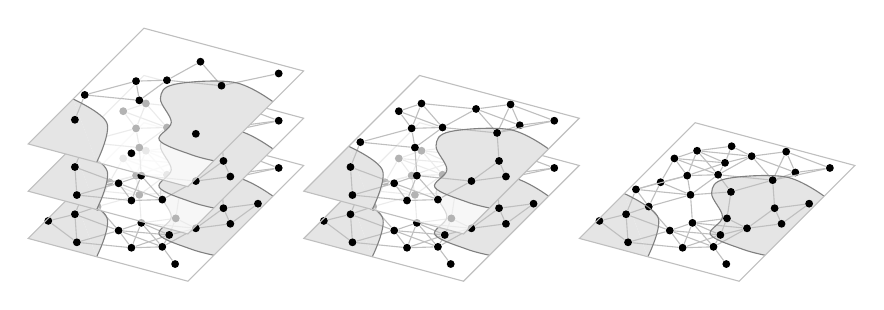
\begin{tikzpicture}

   % left one
   % middle one
   \begin{scope}[shift={(0,0)}]
   \begin{scope}[x  = {(-0.15cm,-0.15cm)},
                       y  = {(0.2898cm,-0.0776cm)},
                       z  = {(0cm,0.30cm)},
                       scale = 2,
                       color = {lightgray}]
   
   % bottom face
   \begin{scope}[canvas is xy plane at z=0]
      
      % obstacle 1 fill
      \fill[black!10] plot [smooth,tension=0.6] coordinates {
         (1.3,3.5) (1.0,2.5) (1.6,1.5) (2.2,1.5)
         (2.9,2.1) (3.6,2.2) (3.8,3.0) (3.8,3.5)};

      % obstacle 2 fill
      \fill[black!10] plot [smooth,tension=0.6] coordinates {
         (3.0,0.0) (3.5,1.0) (4.9,1.5)};
      \fill[black!10] (4.9,1.5) -- (4.9,0.0) -- (3.0,0.0) -- cycle;

      % graph!
      % $ rosrun ompl_lemur generate-roadmap --dim=2 --bounds=0:0,4.9 --bounds=1:0,3.5 --roadmap-type=Halton --roadmap-param=num=30 --roadmap-param=radius=1.0 --num-batches=1 --out-file=blah.graphio --out-format=graphio
      \node[inner sep=1pt,fill=black,circle] (v0) at (2.45,1.1666666666666665) {};
      \node[inner sep=1pt,fill=black,circle] (v1) at (1.225,2.333333333333333) {};
      \node[inner sep=1pt,fill=black,circle] (v2) at (3.6750000000000003,0.38888888888888884) {};
      \node[inner sep=1pt,fill=black,circle] (v3) at (0.6125,1.5555555555555554) {};
      \node[inner sep=1pt,fill=black,circle] (v4) at (3.0625,2.722222222222222) {};
      \node[inner sep=1pt,fill=black,circle] (v5) at (1.8375000000000001,0.7777777777777777) {};
      \node[inner sep=1pt,fill=black,circle] (v6) at (4.2875000000000005,1.9444444444444446) {};
      \node[inner sep=1pt,fill=black,circle] (v7) at (0.30625,3.1111111111111107) {};
      \node[inner sep=1pt,fill=black,circle] (v8) at (2.75625,0.12962962962962962) {};
      \node[inner sep=1pt,fill=black,circle] (v9) at (1.53125,1.2962962962962963) {};
      \node[inner sep=1pt,fill=black,circle] (v10) at (3.98125,2.462962962962963) {};
      \node[inner sep=1pt,fill=black,circle] (v11) at (0.9187500000000001,0.5185185185185185) {};
      \node[inner sep=1pt,fill=black,circle] (v12) at (3.3687500000000004,1.6851851851851851) {};
      \node[inner sep=1pt,fill=black,circle] (v13) at (2.1437500000000003,2.851851851851851) {};
      \node[inner sep=1pt,fill=black,circle] (v14) at (4.59375,0.9074074074074073) {};
      \node[inner sep=1pt,fill=black,circle] (v15) at (0.153125,2.074074074074074) {};
      \node[inner sep=1pt,fill=black,circle] (v16) at (2.6031250000000004,3.2407407407407405) {};
      \node[inner sep=1pt,fill=black,circle] (v17) at (1.378125,0.25925925925925924) {};
      \node[inner sep=1pt,fill=black,circle] (v18) at (3.8281250000000004,1.4259259259259258) {};
      \node[inner sep=1pt,fill=black,circle] (v19) at (0.765625,2.5925925925925926) {};
      \node[inner sep=1pt,fill=black,circle] (v20) at (3.215625,0.6481481481481481) {};
      \node[inner sep=1pt,fill=black,circle] (v21) at (1.990625,1.8148148148148147) {};
      \node[inner sep=1pt,fill=black,circle] (v22) at (4.440625000000001,2.981481481481481) {};
      \node[inner sep=1pt,fill=black,circle] (v23) at (0.45937500000000003,1.037037037037037) {};
      \node[inner sep=1pt,fill=black,circle] (v24) at (2.9093750000000003,2.2037037037037037) {};
      \node[inner sep=1pt,fill=black,circle] (v25) at (1.6843750000000002,3.3703703703703702) {};
      \node[inner sep=1pt,fill=black,circle] (v26) at (4.134375,0.043209876543209874) {};
      \node[inner sep=1pt,fill=black,circle] (v27) at (1.0718750000000001,1.2098765432098766) {};
      \node[inner sep=1pt,fill=black,circle] (v28) at (3.521875,2.3765432098765427) {};
      \node[inner sep=1pt,fill=black,circle] (v29) at (2.296875,0.43209876543209874) {};
         
      \draw (v3) -- (v1);
      \draw (v5) -- (v0);
      \draw (v7) -- (v1);
      \draw (v8) -- (v0);
      \draw (v8) -- (v2);
      \draw (v8) -- (v5);
      \draw (v9) -- (v0);
      \draw (v9) -- (v1);
      \draw (v9) -- (v3);
      \draw (v9) -- (v5);
      \draw (v10) -- (v4);
      \draw (v10) -- (v6);
      \draw (v11) -- (v3);
      \draw (v11) -- (v5);
      \draw (v11) -- (v9);
      \draw (v12) -- (v0);
      \draw (v12) -- (v4);
      \draw (v12) -- (v6);
      \draw (v12) -- (v10);
      \draw (v13) -- (v1);
      \draw (v13) -- (v4);
      \draw (v14) -- (v2);
      \draw (v14) -- (v6);
      \draw (v15) -- (v1);
      \draw (v15) -- (v3);
      \draw (v15) -- (v7);
      \draw (v16) -- (v4);
      \draw (v16) -- (v13);
      \draw (v17) -- (v5);
      \draw (v17) -- (v9);
      \draw (v17) -- (v11);
      \draw (v18) -- (v2);
      \draw (v18) -- (v6);
      \draw (v18) -- (v10);
      \draw (v18) -- (v12);
      \draw (v18) -- (v14);
      \draw (v19) -- (v1);
      \draw (v19) -- (v3);
      \draw (v19) -- (v7);
      \draw (v19) -- (v15);
      \draw (v20) -- (v0);
      \draw (v20) -- (v2);
      \draw (v20) -- (v8);
      \draw (v20) -- (v18);
      \draw (v21) -- (v0);
      \draw (v21) -- (v1);
      \draw (v21) -- (v9);
      \draw (v22) -- (v10);
      \draw (v23) -- (v3);
      \draw (v23) -- (v11);
      \draw (v24) -- (v4);
      \draw (v24) -- (v12);
      \draw (v24) -- (v21);
      \draw (v25) -- (v13);
      \draw (v25) -- (v16);
      \draw (v26) -- (v2);
      \draw (v26) -- (v14);
      \draw (v27) -- (v3);
      \draw (v27) -- (v5);
      \draw (v27) -- (v9);
      \draw (v27) -- (v11);
      \draw (v27) -- (v17);
      \draw (v27) -- (v23);
      \draw (v28) -- (v4);
      \draw (v28) -- (v6);
      \draw (v28) -- (v10);
      \draw (v28) -- (v12);
      \draw (v28) -- (v18);
      \draw (v28) -- (v24);
      \draw (v29) -- (v0);
      \draw (v29) -- (v5);
      \draw (v29) -- (v8);
      \draw (v29) -- (v17);
      \draw (v29) -- (v20);



      % obstacle 1 boundary
      \draw[black!50] plot [smooth,tension=0.6] coordinates {
         (1.3,3.5) (1.0,2.5) (1.6,1.5) (2.2,1.5)
         (2.9,2.1) (3.6,2.2) (3.8,3.0) (3.8,3.5)};

      % obstacle 2 boundary
      \draw[black!50] plot [smooth,tension=0.6] coordinates {
         (3.0,0.0) (3.5,1.0) (4.9,1.5)};

      % path
      %\draw plot [smooth,tension=0.6,thick] coordinates {
      %   (0.5,2.0) (1.0,1.0) (2.8,1.0) (4.0,1.9) (4.4,2.2)};

      % path endpoints / labels
      %\fill[black] (0.5,2.0) circle (0.05cm);
      %\fill[black] (4.4,2.2) circle (0.05cm);
      
      % C-space border
      \draw (0,0) -- (0,3.5) -- (4.9,3.5) -- (4.9,0) -- cycle;
      
   \end{scope}
   
   
   
   % middle face
   \begin{scope}[canvas is xy plane at z=1]
      
      \fill[color=white,opacity=0.7] (0,0) -- (0,3.5) -- (4.9,3.5) -- (4.9,0) -- cycle;
      
      % obstacle 1 fill
      \fill[black!10] plot [smooth,tension=0.6] coordinates {
         (1.3,3.5) (1.0,2.5) (1.6,1.5) (2.2,1.5)
         (2.9,2.1) (3.6,2.2) (3.8,3.0) (3.8,3.5)};

      % obstacle 2 fill
      \fill[black!10] plot [smooth,tension=0.6] coordinates {
         (3.0,0.0) (3.5,1.0) (4.9,1.5)};
      \fill[black!10] (4.9,1.5) -- (4.9,0.0) -- (3.0,0.0) -- cycle;


      % $ rosrun ompl_lemur generate-roadmap --dim=2 --bounds=0:0,4.9 --bounds=1:0,3.5 --roadmap-type=Halton --roadmap-param=num=20 --roadmap-param=radius=1.2 --num-batches=1 --out-file=blah.graphio --out-format=graphio
      \node[inner sep=1pt,fill=black,circle] (v0) at (2.45,1.1666666666666665) {};
      \node[inner sep=1pt,fill=black,circle] (v1) at (1.225,2.333333333333333) {};
      \node[inner sep=1pt,fill=black,circle] (v2) at (3.6750000000000003,0.38888888888888884) {};
      \node[inner sep=1pt,fill=black,circle] (v3) at (0.6125,1.5555555555555554) {};
      \node[inner sep=1pt,fill=black,circle] (v4) at (3.0625,2.722222222222222) {};
      \node[inner sep=1pt,fill=black,circle] (v5) at (1.8375000000000001,0.7777777777777777) {};
      \node[inner sep=1pt,fill=black,circle] (v6) at (4.2875000000000005,1.9444444444444446) {};
      \node[inner sep=1pt,fill=black,circle] (v7) at (0.30625,3.1111111111111107) {};
      \node[inner sep=1pt,fill=black,circle] (v8) at (2.75625,0.12962962962962962) {};
      \node[inner sep=1pt,fill=black,circle] (v9) at (1.53125,1.2962962962962963) {};
      \node[inner sep=1pt,fill=black,circle] (v10) at (3.98125,2.462962962962963) {};
      \node[inner sep=1pt,fill=black,circle] (v11) at (0.9187500000000001,0.5185185185185185) {};
      \node[inner sep=1pt,fill=black,circle] (v12) at (3.3687500000000004,1.6851851851851851) {};
      \node[inner sep=1pt,fill=black,circle] (v13) at (2.1437500000000003,2.851851851851851) {};
      \node[inner sep=1pt,fill=black,circle] (v14) at (4.59375,0.9074074074074073) {};
      \node[inner sep=1pt,fill=black,circle] (v15) at (0.153125,2.074074074074074) {};
      \node[inner sep=1pt,fill=black,circle] (v16) at (2.6031250000000004,3.2407407407407405) {};
      \node[inner sep=1pt,fill=black,circle] (v17) at (1.378125,0.25925925925925924) {};
      \node[inner sep=1pt,fill=black,circle] (v18) at (3.8281250000000004,1.4259259259259258) {};
      \node[inner sep=1pt,fill=black,circle] (v19) at (0.765625,2.5925925925925926) {};



      \draw (v3) -- (v1);
      \draw (v5) -- (v0);
      \draw (v7) -- (v1);
      \draw (v8) -- (v0);
      \draw (v8) -- (v2);
      \draw (v8) -- (v5);
      \draw (v9) -- (v0);
      \draw (v9) -- (v1);
      \draw (v9) -- (v3);
      \draw (v9) -- (v5);
      \draw (v10) -- (v4);
      \draw (v10) -- (v6);
      \draw (v11) -- (v3);
      \draw (v11) -- (v5);
      \draw (v11) -- (v9);
      \draw (v12) -- (v0);
      \draw (v12) -- (v4);
      \draw (v12) -- (v6);
      \draw (v12) -- (v10);
      \draw (v13) -- (v1);
      \draw (v13) -- (v4);
      \draw (v14) -- (v2);
      \draw (v14) -- (v6);
      \draw (v15) -- (v1);
      \draw (v15) -- (v3);
      \draw (v15) -- (v7);
      \draw (v16) -- (v4);
      \draw (v16) -- (v13);
      \draw (v17) -- (v5);
      \draw (v17) -- (v9);
      \draw (v17) -- (v11);
      \draw (v18) -- (v2);
      \draw (v18) -- (v6);
      \draw (v18) -- (v10);
      \draw (v18) -- (v12);
      \draw (v18) -- (v14);
      \draw (v19) -- (v1);
      \draw (v19) -- (v3);
      \draw (v19) -- (v7);
      \draw (v19) -- (v15);


      % obstacle 1 boundary
      \draw[black!50] plot [smooth,tension=0.6] coordinates {
         (1.3,3.5) (1.0,2.5) (1.6,1.5) (2.2,1.5)
         (2.9,2.1) (3.6,2.2) (3.8,3.0) (3.8,3.5)};

      % obstacle 2 boundary
      \draw[black!50] plot [smooth,tension=0.6] coordinates {
         (3.0,0.0) (3.5,1.0) (4.9,1.5)};

      % path
      %\draw plot [smooth,tension=0.6,thick] coordinates {
      %   (0.5,2.0) (1.0,1.0) (2.8,1.0) (4.0,1.9) (4.4,2.2)};

      % path endpoints / labels
      %\fill[black] (0.5,2.0) circle (0.05cm);
      %\fill[black] (4.4,2.2) circle (0.05cm);
      
      % C-space border
      \draw (0,0) -- (0,3.5) -- (4.9,3.5) -- (4.9,0) -- cycle;
      
   \end{scope}
   
   
   % top face
   \begin{scope}[canvas is xy plane at z=2]
      \fill[color=white,opacity=0.7] (0,0) -- (0,3.5) -- (4.9,3.5) -- (4.9,0) -- cycle;
      % obstacle 1 fill
      \fill[black!10] plot [smooth,tension=0.6] coordinates {
         (1.3,3.5) (1.0,2.5) (1.6,1.5) (2.2,1.5)
         (2.9,2.1) (3.6,2.2) (3.8,3.0) (3.8,3.5)};
      % obstacle 2 fill
      \fill[black!10] plot [smooth,tension=0.6] coordinates {
         (3.0,0.0) (3.5,1.0) (4.9,1.5)};
      \fill[black!10] (4.9,1.5) -- (4.9,0.0) -- (3.0,0.0) -- cycle;

      % $ rosrun ompl_lemur generate-roadmap --dim=2 --bounds=0:0,4.9 --bounds=1:0,3.5 --roadmap-type=Halton --roadmap-param=num=10 --roadmap-param=radius=1.4 --num-batches=1 --out-file=blah.graphio --out-format=graphio
      \node[inner sep=1pt,fill=black,circle] (v0) at (2.45,1.1666666666666665) {};
      \node[inner sep=1pt,fill=black,circle] (v1) at (1.225,2.333333333333333) {};
      \node[inner sep=1pt,fill=black,circle] (v2) at (3.6750000000000003,0.38888888888888884) {};
      \node[inner sep=1pt,fill=black,circle] (v3) at (0.6125,1.5555555555555554) {};
      \node[inner sep=1pt,fill=black,circle] (v4) at (3.0625,2.722222222222222) {};
      \node[inner sep=1pt,fill=black,circle] (v5) at (1.8375000000000001,0.7777777777777777) {};
      \node[inner sep=1pt,fill=black,circle] (v6) at (4.2875000000000005,1.9444444444444446) {};
      \node[inner sep=1pt,fill=black,circle] (v7) at (0.30625,3.1111111111111107) {};
      \node[inner sep=1pt,fill=black,circle] (v8) at (2.75625,0.12962962962962962) {};
      \node[inner sep=1pt,fill=black,circle] (v9) at (1.53125,1.2962962962962963) {};
      \draw (v3) -- (v1);
      \draw (v5) -- (v0);
      \draw (v7) -- (v1);
      \draw (v8) -- (v0);
      \draw (v8) -- (v2);
      \draw (v8) -- (v5);
      \draw (v9) -- (v0);
      \draw (v9) -- (v1);
      \draw (v9) -- (v3);
      \draw (v9) -- (v5);
      
      % obstacle 1 boundary
      \draw[black!50] plot [smooth,tension=0.6] coordinates {
         (1.3,3.5) (1.0,2.5) (1.6,1.5) (2.2,1.5)
         (2.9,2.1) (3.6,2.2) (3.8,3.0) (3.8,3.5)};
      % obstacle 2 boundary
      \draw[black!50] plot [smooth,tension=0.6] coordinates {
         (3.0,0.0) (3.5,1.0) (4.9,1.5)};
      % C-space border
      \draw (0,0) -- (0,3.5) -- (4.9,3.5) -- (4.9,0) -- cycle;
   \end{scope}

   \end{scope}
   \end{scope}




   % middle one
   \begin{scope}[shift={(3.5,0)}]
   \begin{scope}[x  = {(-0.15cm,-0.15cm)},
                       y  = {(0.2898cm,-0.0776cm)},
                       z  = {(0cm,0.30cm)},
                       scale = 2,
                       color = {lightgray}]
   
   % bottom face
   \begin{scope}[canvas is xy plane at z=0]
      
      % obstacle 1 fill
      \fill[black!10] plot [smooth,tension=0.6] coordinates {
         (1.3,3.5) (1.0,2.5) (1.6,1.5) (2.2,1.5)
         (2.9,2.1) (3.6,2.2) (3.8,3.0) (3.8,3.5)};

      % obstacle 2 fill
      \fill[black!10] plot [smooth,tension=0.6] coordinates {
         (3.0,0.0) (3.5,1.0) (4.9,1.5)};
      \fill[black!10] (4.9,1.5) -- (4.9,0.0) -- (3.0,0.0) -- cycle;

      % graph!
      % $ rosrun ompl_lemur generate-roadmap --dim=2 --bounds=0:0,4.9 --bounds=1:0,3.5 --roadmap-type=Halton --roadmap-param=num=30 --roadmap-param=radius=1.0 --num-batches=1 --out-file=blah.graphio --out-format=graphio
      \node[inner sep=1pt,fill=black,circle] (v0) at (2.45,1.1666666666666665) {};
      \node[inner sep=1pt,fill=black,circle] (v1) at (1.225,2.333333333333333) {};
      \node[inner sep=1pt,fill=black,circle] (v2) at (3.6750000000000003,0.38888888888888884) {};
      \node[inner sep=1pt,fill=black,circle] (v3) at (0.6125,1.5555555555555554) {};
      \node[inner sep=1pt,fill=black,circle] (v4) at (3.0625,2.722222222222222) {};
      \node[inner sep=1pt,fill=black,circle] (v5) at (1.8375000000000001,0.7777777777777777) {};
      \node[inner sep=1pt,fill=black,circle] (v6) at (4.2875000000000005,1.9444444444444446) {};
      \node[inner sep=1pt,fill=black,circle] (v7) at (0.30625,3.1111111111111107) {};
      \node[inner sep=1pt,fill=black,circle] (v8) at (2.75625,0.12962962962962962) {};
      \node[inner sep=1pt,fill=black,circle] (v9) at (1.53125,1.2962962962962963) {};
      \node[inner sep=1pt,fill=black,circle] (v10) at (3.98125,2.462962962962963) {};
      \node[inner sep=1pt,fill=black,circle] (v11) at (0.9187500000000001,0.5185185185185185) {};
      \node[inner sep=1pt,fill=black,circle] (v12) at (3.3687500000000004,1.6851851851851851) {};
      \node[inner sep=1pt,fill=black,circle] (v13) at (2.1437500000000003,2.851851851851851) {};
      \node[inner sep=1pt,fill=black,circle] (v14) at (4.59375,0.9074074074074073) {};
      \node[inner sep=1pt,fill=black,circle] (v15) at (0.153125,2.074074074074074) {};
      \node[inner sep=1pt,fill=black,circle] (v16) at (2.6031250000000004,3.2407407407407405) {};
      \node[inner sep=1pt,fill=black,circle] (v17) at (1.378125,0.25925925925925924) {};
      \node[inner sep=1pt,fill=black,circle] (v18) at (3.8281250000000004,1.4259259259259258) {};
      \node[inner sep=1pt,fill=black,circle] (v19) at (0.765625,2.5925925925925926) {};
      \node[inner sep=1pt,fill=black,circle] (v20) at (3.215625,0.6481481481481481) {};
      \node[inner sep=1pt,fill=black,circle] (v21) at (1.990625,1.8148148148148147) {};
      \node[inner sep=1pt,fill=black,circle] (v22) at (4.440625000000001,2.981481481481481) {};
      \node[inner sep=1pt,fill=black,circle] (v23) at (0.45937500000000003,1.037037037037037) {};
      \node[inner sep=1pt,fill=black,circle] (v24) at (2.9093750000000003,2.2037037037037037) {};
      \node[inner sep=1pt,fill=black,circle] (v25) at (1.6843750000000002,3.3703703703703702) {};
      \node[inner sep=1pt,fill=black,circle] (v26) at (4.134375,0.043209876543209874) {};
      \node[inner sep=1pt,fill=black,circle] (v27) at (1.0718750000000001,1.2098765432098766) {};
      \node[inner sep=1pt,fill=black,circle] (v28) at (3.521875,2.3765432098765427) {};
      \node[inner sep=1pt,fill=black,circle] (v29) at (2.296875,0.43209876543209874) {};
         
      \draw (v3) -- (v1);
      \draw (v5) -- (v0);
      \draw (v7) -- (v1);
      \draw (v8) -- (v0);
      \draw (v8) -- (v2);
      \draw (v8) -- (v5);
      \draw (v9) -- (v0);
      \draw (v9) -- (v1);
      \draw (v9) -- (v3);
      \draw (v9) -- (v5);
      \draw (v10) -- (v4);
      \draw (v10) -- (v6);
      \draw (v11) -- (v3);
      \draw (v11) -- (v5);
      \draw (v11) -- (v9);
      \draw (v12) -- (v0);
      \draw (v12) -- (v4);
      \draw (v12) -- (v6);
      \draw (v12) -- (v10);
      \draw (v13) -- (v1);
      \draw (v13) -- (v4);
      \draw (v14) -- (v2);
      \draw (v14) -- (v6);
      \draw (v15) -- (v1);
      \draw (v15) -- (v3);
      \draw (v15) -- (v7);
      \draw (v16) -- (v4);
      \draw (v16) -- (v13);
      \draw (v17) -- (v5);
      \draw (v17) -- (v9);
      \draw (v17) -- (v11);
      \draw (v18) -- (v2);
      \draw (v18) -- (v6);
      \draw (v18) -- (v10);
      \draw (v18) -- (v12);
      \draw (v18) -- (v14);
      \draw (v19) -- (v1);
      \draw (v19) -- (v3);
      \draw (v19) -- (v7);
      \draw (v19) -- (v15);
      \draw (v20) -- (v0);
      \draw (v20) -- (v2);
      \draw (v20) -- (v8);
      \draw (v20) -- (v18);
      \draw (v21) -- (v0);
      \draw (v21) -- (v1);
      \draw (v21) -- (v9);
      \draw (v22) -- (v10);
      \draw (v23) -- (v3);
      \draw (v23) -- (v11);
      \draw (v24) -- (v4);
      \draw (v24) -- (v12);
      \draw (v24) -- (v21);
      \draw (v25) -- (v13);
      \draw (v25) -- (v16);
      \draw (v26) -- (v2);
      \draw (v26) -- (v14);
      \draw (v27) -- (v3);
      \draw (v27) -- (v5);
      \draw (v27) -- (v9);
      \draw (v27) -- (v11);
      \draw (v27) -- (v17);
      \draw (v27) -- (v23);
      \draw (v28) -- (v4);
      \draw (v28) -- (v6);
      \draw (v28) -- (v10);
      \draw (v28) -- (v12);
      \draw (v28) -- (v18);
      \draw (v28) -- (v24);
      \draw (v29) -- (v0);
      \draw (v29) -- (v5);
      \draw (v29) -- (v8);
      \draw (v29) -- (v17);
      \draw (v29) -- (v20);



      % obstacle 1 boundary
      \draw[black!50] plot [smooth,tension=0.6] coordinates {
         (1.3,3.5) (1.0,2.5) (1.6,1.5) (2.2,1.5)
         (2.9,2.1) (3.6,2.2) (3.8,3.0) (3.8,3.5)};

      % obstacle 2 boundary
      \draw[black!50] plot [smooth,tension=0.6] coordinates {
         (3.0,0.0) (3.5,1.0) (4.9,1.5)};

      % path
      %\draw plot [smooth,tension=0.6,thick] coordinates {
      %   (0.5,2.0) (1.0,1.0) (2.8,1.0) (4.0,1.9) (4.4,2.2)};

      % path endpoints / labels
      %\fill[black] (0.5,2.0) circle (0.05cm);
      %\fill[black] (4.4,2.2) circle (0.05cm);
      
      % C-space border
      \draw (0,0) -- (0,3.5) -- (4.9,3.5) -- (4.9,0) -- cycle;
      
   \end{scope}
   
   
   
   % middle face
   \begin{scope}[canvas is xy plane at z=1]
      
      \fill[color=white,opacity=0.7] (0,0) -- (0,3.5) -- (4.9,3.5) -- (4.9,0) -- cycle;
      
      % obstacle 1 fill
      \fill[black!10] plot [smooth,tension=0.6] coordinates {
         (1.3,3.5) (1.0,2.5) (1.6,1.5) (2.2,1.5)
         (2.9,2.1) (3.6,2.2) (3.8,3.0) (3.8,3.5)};

      % obstacle 2 fill
      \fill[black!10] plot [smooth,tension=0.6] coordinates {
         (3.0,0.0) (3.5,1.0) (4.9,1.5)};
      \fill[black!10] (4.9,1.5) -- (4.9,0.0) -- (3.0,0.0) -- cycle;


      % $ rosrun ompl_lemur generate-roadmap --dim=2 --bounds=0:0,4.9 --bounds=1:0,3.5 --roadmap-type=Halton --roadmap-param=num=20 --roadmap-param=radius=1.2 --num-batches=1 --out-file=blah.graphio --out-format=graphio
      \node[inner sep=1pt,fill=black,circle] (v0) at (2.45,1.1666666666666665) {};
      \node[inner sep=1pt,fill=black,circle] (v1) at (1.225,2.333333333333333) {};
      \node[inner sep=1pt,fill=black,circle] (v2) at (3.6750000000000003,0.38888888888888884) {};
      \node[inner sep=1pt,fill=black,circle] (v3) at (0.6125,1.5555555555555554) {};
      \node[inner sep=1pt,fill=black,circle] (v4) at (3.0625,2.722222222222222) {};
      \node[inner sep=1pt,fill=black,circle] (v5) at (1.8375000000000001,0.7777777777777777) {};
      \node[inner sep=1pt,fill=black,circle] (v6) at (4.2875000000000005,1.9444444444444446) {};
      \node[inner sep=1pt,fill=black,circle] (v7) at (0.30625,3.1111111111111107) {};
      \node[inner sep=1pt,fill=black,circle] (v8) at (2.75625,0.12962962962962962) {};
      \node[inner sep=1pt,fill=black,circle] (v9) at (1.53125,1.2962962962962963) {};
      \node[inner sep=1pt,fill=black,circle] (v10) at (3.98125,2.462962962962963) {};
      \node[inner sep=1pt,fill=black,circle] (v11) at (0.9187500000000001,0.5185185185185185) {};
      \node[inner sep=1pt,fill=black,circle] (v12) at (3.3687500000000004,1.6851851851851851) {};
      \node[inner sep=1pt,fill=black,circle] (v13) at (2.1437500000000003,2.851851851851851) {};
      \node[inner sep=1pt,fill=black,circle] (v14) at (4.59375,0.9074074074074073) {};
      \node[inner sep=1pt,fill=black,circle] (v15) at (0.153125,2.074074074074074) {};
      \node[inner sep=1pt,fill=black,circle] (v16) at (2.6031250000000004,3.2407407407407405) {};
      \node[inner sep=1pt,fill=black,circle] (v17) at (1.378125,0.25925925925925924) {};
      \node[inner sep=1pt,fill=black,circle] (v18) at (3.8281250000000004,1.4259259259259258) {};
      \node[inner sep=1pt,fill=black,circle] (v19) at (0.765625,2.5925925925925926) {};



      \draw (v3) -- (v1);
      \draw (v5) -- (v0);
      \draw (v7) -- (v1);
      \draw (v8) -- (v0);
      \draw (v8) -- (v2);
      \draw (v8) -- (v5);
      \draw (v9) -- (v0);
      \draw (v9) -- (v1);
      \draw (v9) -- (v3);
      \draw (v9) -- (v5);
      \draw (v10) -- (v4);
      \draw (v10) -- (v6);
      \draw (v11) -- (v3);
      \draw (v11) -- (v5);
      \draw (v11) -- (v9);
      \draw (v12) -- (v0);
      \draw (v12) -- (v4);
      \draw (v12) -- (v6);
      \draw (v12) -- (v10);
      \draw (v13) -- (v1);
      \draw (v13) -- (v4);
      \draw (v14) -- (v2);
      \draw (v14) -- (v6);
      \draw (v15) -- (v1);
      \draw (v15) -- (v3);
      \draw (v15) -- (v7);
      \draw (v16) -- (v4);
      \draw (v16) -- (v13);
      \draw (v17) -- (v5);
      \draw (v17) -- (v9);
      \draw (v17) -- (v11);
      \draw (v18) -- (v2);
      \draw (v18) -- (v6);
      \draw (v18) -- (v10);
      \draw (v18) -- (v12);
      \draw (v18) -- (v14);
      \draw (v19) -- (v1);
      \draw (v19) -- (v3);
      \draw (v19) -- (v7);
      \draw (v19) -- (v15);


      % obstacle 1 boundary
      \draw[black!50] plot [smooth,tension=0.6] coordinates {
         (1.3,3.5) (1.0,2.5) (1.6,1.5) (2.2,1.5)
         (2.9,2.1) (3.6,2.2) (3.8,3.0) (3.8,3.5)};

      % obstacle 2 boundary
      \draw[black!50] plot [smooth,tension=0.6] coordinates {
         (3.0,0.0) (3.5,1.0) (4.9,1.5)};

      % path
      %\draw plot [smooth,tension=0.6,thick] coordinates {
      %   (0.5,2.0) (1.0,1.0) (2.8,1.0) (4.0,1.9) (4.4,2.2)};

      % path endpoints / labels
      %\fill[black] (0.5,2.0) circle (0.05cm);
      %\fill[black] (4.4,2.2) circle (0.05cm);
      
      % C-space border
      \draw (0,0) -- (0,3.5) -- (4.9,3.5) -- (4.9,0) -- cycle;
      
   \end{scope}
   
   \end{scope}
   \end{scope}




   % right one
   \begin{scope}[shift={(7,0)}]
   \begin{scope}[x  = {(-0.15cm,-0.15cm)},
                       y  = {(0.2898cm,-0.0776cm)},
                       z  = {(0cm,0.30cm)},
                       scale = 2,
                       color = {lightgray}]
   
   % bottom face
   \begin{scope}[canvas is xy plane at z=0]
      
      % obstacle 1 fill
      \fill[black!10] plot [smooth,tension=0.6] coordinates {
         (1.3,3.5) (1.0,2.5) (1.6,1.5) (2.2,1.5)
         (2.9,2.1) (3.6,2.2) (3.8,3.0) (3.8,3.5)};

      % obstacle 2 fill
      \fill[black!10] plot [smooth,tension=0.6] coordinates {
         (3.0,0.0) (3.5,1.0) (4.9,1.5)};
      \fill[black!10] (4.9,1.5) -- (4.9,0.0) -- (3.0,0.0) -- cycle;

      % graph!
      % $ rosrun ompl_lemur generate-roadmap --dim=2 --bounds=0:0,4.9 --bounds=1:0,3.5 --roadmap-type=Halton --roadmap-param=num=30 --roadmap-param=radius=1.0 --num-batches=1 --out-file=blah.graphio --out-format=graphio
      \node[inner sep=1pt,fill=black,circle] (v0) at (2.45,1.1666666666666665) {};
      \node[inner sep=1pt,fill=black,circle] (v1) at (1.225,2.333333333333333) {};
      \node[inner sep=1pt,fill=black,circle] (v2) at (3.6750000000000003,0.38888888888888884) {};
      \node[inner sep=1pt,fill=black,circle] (v3) at (0.6125,1.5555555555555554) {};
      \node[inner sep=1pt,fill=black,circle] (v4) at (3.0625,2.722222222222222) {};
      \node[inner sep=1pt,fill=black,circle] (v5) at (1.8375000000000001,0.7777777777777777) {};
      \node[inner sep=1pt,fill=black,circle] (v6) at (4.2875000000000005,1.9444444444444446) {};
      \node[inner sep=1pt,fill=black,circle] (v7) at (0.30625,3.1111111111111107) {};
      \node[inner sep=1pt,fill=black,circle] (v8) at (2.75625,0.12962962962962962) {};
      \node[inner sep=1pt,fill=black,circle] (v9) at (1.53125,1.2962962962962963) {};
      \node[inner sep=1pt,fill=black,circle] (v10) at (3.98125,2.462962962962963) {};
      \node[inner sep=1pt,fill=black,circle] (v11) at (0.9187500000000001,0.5185185185185185) {};
      \node[inner sep=1pt,fill=black,circle] (v12) at (3.3687500000000004,1.6851851851851851) {};
      \node[inner sep=1pt,fill=black,circle] (v13) at (2.1437500000000003,2.851851851851851) {};
      \node[inner sep=1pt,fill=black,circle] (v14) at (4.59375,0.9074074074074073) {};
      \node[inner sep=1pt,fill=black,circle] (v15) at (0.153125,2.074074074074074) {};
      \node[inner sep=1pt,fill=black,circle] (v16) at (2.6031250000000004,3.2407407407407405) {};
      \node[inner sep=1pt,fill=black,circle] (v17) at (1.378125,0.25925925925925924) {};
      \node[inner sep=1pt,fill=black,circle] (v18) at (3.8281250000000004,1.4259259259259258) {};
      \node[inner sep=1pt,fill=black,circle] (v19) at (0.765625,2.5925925925925926) {};
      \node[inner sep=1pt,fill=black,circle] (v20) at (3.215625,0.6481481481481481) {};
      \node[inner sep=1pt,fill=black,circle] (v21) at (1.990625,1.8148148148148147) {};
      \node[inner sep=1pt,fill=black,circle] (v22) at (4.440625000000001,2.981481481481481) {};
      \node[inner sep=1pt,fill=black,circle] (v23) at (0.45937500000000003,1.037037037037037) {};
      \node[inner sep=1pt,fill=black,circle] (v24) at (2.9093750000000003,2.2037037037037037) {};
      \node[inner sep=1pt,fill=black,circle] (v25) at (1.6843750000000002,3.3703703703703702) {};
      \node[inner sep=1pt,fill=black,circle] (v26) at (4.134375,0.043209876543209874) {};
      \node[inner sep=1pt,fill=black,circle] (v27) at (1.0718750000000001,1.2098765432098766) {};
      \node[inner sep=1pt,fill=black,circle] (v28) at (3.521875,2.3765432098765427) {};
      \node[inner sep=1pt,fill=black,circle] (v29) at (2.296875,0.43209876543209874) {};
         
      \draw (v3) -- (v1);
      \draw (v5) -- (v0);
      \draw (v7) -- (v1);
      \draw (v8) -- (v0);
      \draw (v8) -- (v2);
      \draw (v8) -- (v5);
      \draw (v9) -- (v0);
      \draw (v9) -- (v1);
      \draw (v9) -- (v3);
      \draw (v9) -- (v5);
      \draw (v10) -- (v4);
      \draw (v10) -- (v6);
      \draw (v11) -- (v3);
      \draw (v11) -- (v5);
      \draw (v11) -- (v9);
      \draw (v12) -- (v0);
      \draw (v12) -- (v4);
      \draw (v12) -- (v6);
      \draw (v12) -- (v10);
      \draw (v13) -- (v1);
      \draw (v13) -- (v4);
      \draw (v14) -- (v2);
      \draw (v14) -- (v6);
      \draw (v15) -- (v1);
      \draw (v15) -- (v3);
      \draw (v15) -- (v7);
      \draw (v16) -- (v4);
      \draw (v16) -- (v13);
      \draw (v17) -- (v5);
      \draw (v17) -- (v9);
      \draw (v17) -- (v11);
      \draw (v18) -- (v2);
      \draw (v18) -- (v6);
      \draw (v18) -- (v10);
      \draw (v18) -- (v12);
      \draw (v18) -- (v14);
      \draw (v19) -- (v1);
      \draw (v19) -- (v3);
      \draw (v19) -- (v7);
      \draw (v19) -- (v15);
      \draw (v20) -- (v0);
      \draw (v20) -- (v2);
      \draw (v20) -- (v8);
      \draw (v20) -- (v18);
      \draw (v21) -- (v0);
      \draw (v21) -- (v1);
      \draw (v21) -- (v9);
      \draw (v22) -- (v10);
      \draw (v23) -- (v3);
      \draw (v23) -- (v11);
      \draw (v24) -- (v4);
      \draw (v24) -- (v12);
      \draw (v24) -- (v21);
      \draw (v25) -- (v13);
      \draw (v25) -- (v16);
      \draw (v26) -- (v2);
      \draw (v26) -- (v14);
      \draw (v27) -- (v3);
      \draw (v27) -- (v5);
      \draw (v27) -- (v9);
      \draw (v27) -- (v11);
      \draw (v27) -- (v17);
      \draw (v27) -- (v23);
      \draw (v28) -- (v4);
      \draw (v28) -- (v6);
      \draw (v28) -- (v10);
      \draw (v28) -- (v12);
      \draw (v28) -- (v18);
      \draw (v28) -- (v24);
      \draw (v29) -- (v0);
      \draw (v29) -- (v5);
      \draw (v29) -- (v8);
      \draw (v29) -- (v17);
      \draw (v29) -- (v20);



      % obstacle 1 boundary
      \draw[black!50] plot [smooth,tension=0.6] coordinates {
         (1.3,3.5) (1.0,2.5) (1.6,1.5) (2.2,1.5)
         (2.9,2.1) (3.6,2.2) (3.8,3.0) (3.8,3.5)};

      % obstacle 2 boundary
      \draw[black!50] plot [smooth,tension=0.6] coordinates {
         (3.0,0.0) (3.5,1.0) (4.9,1.5)};

      % path
      %\draw plot [smooth,tension=0.6,thick] coordinates {
      %   (0.5,2.0) (1.0,1.0) (2.8,1.0) (4.0,1.9) (4.4,2.2)};

      % path endpoints / labels
      %\fill[black] (0.5,2.0) circle (0.05cm);
      %\fill[black] (4.4,2.2) circle (0.05cm);
      
      % C-space border
      \draw (0,0) -- (0,3.5) -- (4.9,3.5) -- (4.9,0) -- cycle;
      
   \end{scope}

   \end{scope}
   \end{scope}

\end{tikzpicture}%
\end{document}
